\subsection{Making Routers Observable and Controllable:  Router Boundary Scan}

\paragraph*{Task:} (Challenge C9, Netravali, Tamir, Varghese).  Many faults in routers are caused not by configuration 
problems but by microde or hardware bugs that are hard to isolate because it is difficult to send test inputs to 
operational routers to diagnose the problem. Imagine that we could send a  Voice over IP packet between two routers in the middle
of the network to test whether its being delayed in a queue at either router.  Or to send a BGP annoucement to only one router to
manupulate its Routing Table?  Imagine that we could also observe the state of the routers after each such packet.  Then routers
would become {\em controllable} and {\em observable}.

\paragraph*{Science:} Past work~\cite{jtag} in {\em hardware boundary scan} (implemented in a standard popularly known as JTAG) allows hardware modules (e.g., chips) to be sent arbitrary test input (Figure~\ref{rtagfigure}) and the output 
fron the same module to be read out by the tester without having physical wires from the tester to each chip.  Inspired
by this idea, we propose {\em router boundary scan} to allow a tester to send an {\em arbitrary packet} (e.g., an application
packet or even a router announcement) to an {\em arbitrary} router to be sent out on an arbitrary interface, and having the 
router hardware snapshot state at the receiving and sending ends that can be later collected by the tester.

\paragraph*{Approach:} If we consider a router as a module, we are looking to send arbitary test inputs to the router and
observe the results.  Software module testing is comparitively easy because we can typically isolate a software module in
a test harness.  However, in hardware, if the system is a board and the ``modules'' are chips, it is often difficult to find 
the right set of board inputs to send appropriate test signals to a specified chip.  Wires from the tester to each chip would
work but this would grreatly increase the number of pins.  Instead, in hardware boundary scan, (Figure~\ref{rtagfigure}) a few
 shared JTAG pins are reserved for testing and the test inputs is connected to a daisy chain serial network that reaches all
 pins.  The test input for say a chip $C2$ can then be shifted through the prior chips in the daisy chain network till it
 reaches $C2$.  A similar daisy chain network is used to collect the output from $C2$.
 
 \begin{figure*}[t]
\centering
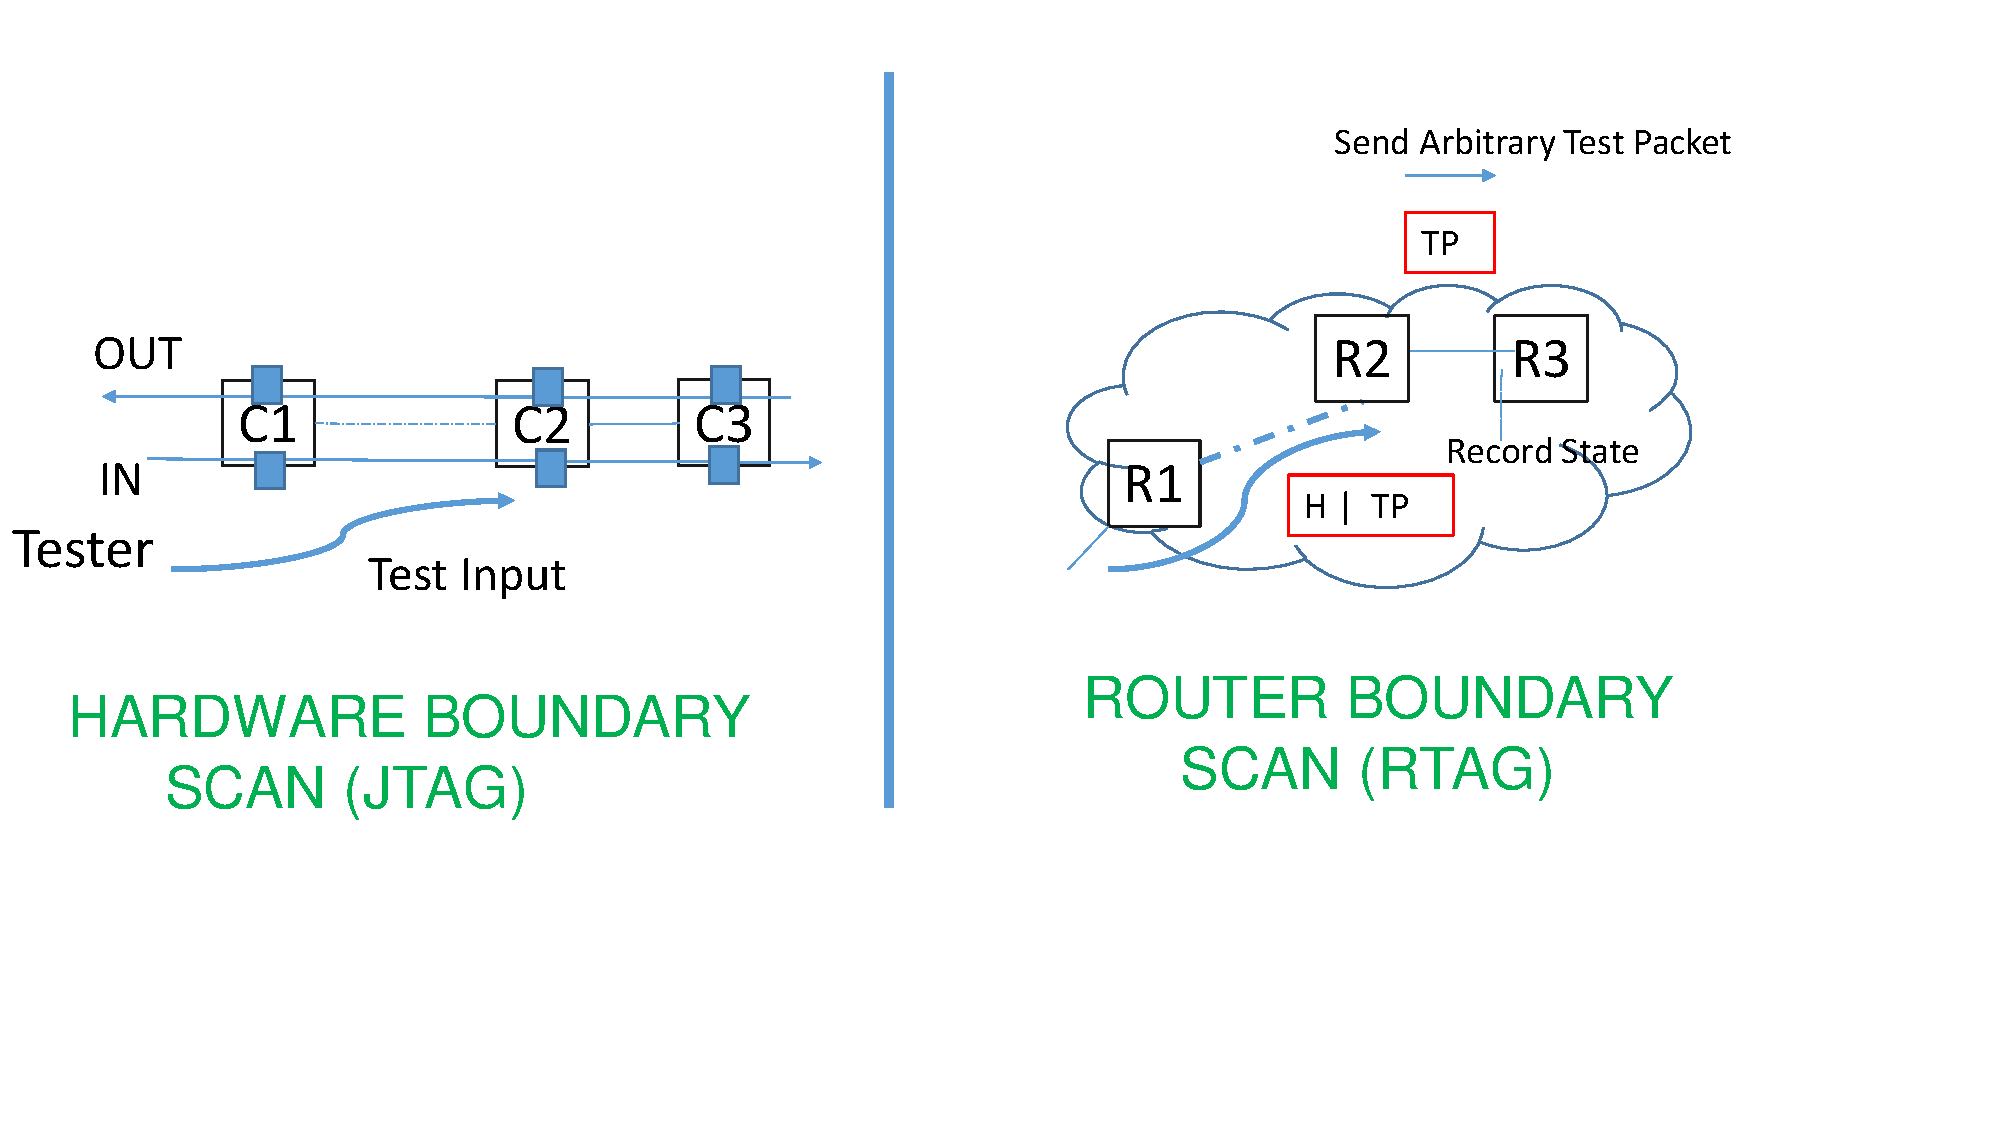
\includegraphics[width=0.7\textwidth]{RTAG.pdf}
\caption{Overview of our proposal to automatically bridge the gap between
operator/developer concerns and low-level tracing systems.}
\label{fig:rtagfigure}
\end{figure*}

 Inspired by this, we propose a new router boundary scan mechanism (RTAG for Router Target Action Generation) where an
 external tester can send an arbitrary packet ({\em TP}  on the right of Figure~\ref{rtagfigure}) to an arbitrary router ($R3$) 
 by encapsulating it (using say IP in IP encapsulation) to $R4$ together with control information that specifies which interface
 it must be sent on.  Before sending the test packet {\em TP} the tester ``arms'' the other end of the interface (e.g., $R3$) to
 detect this test packet using a prespecified pattern detection predicate.  Just as in JTAG, we propose that every router add
 new hardware to snapshot state (e.g., time sent/received, queue sizes) on sending/receiving {\em TP} which can later be collected by the
 tester.
 
 We believe that Router Boundary Scan can help real time detection of a number of hard to isolate phenomena we have observed
 in data centers including hardware and microcode bugs, and mysterious packet losses.  Further, we believe this can be combined
 with the network system debugging described in Section~\ref{ravi} to go from operator logs to tester queries to isolation to particular
 routers.  From discussions with Cisco's Tom Edsall\footnote{the chied designer of Cisco's Catalyst Route and their latest Data Center routers}, it appears that such a mechanism is not available in any current router but is feasible to add. Edsall (see letter) is willing to work with us to refine this scheme so
 that its hardware implementation is feasible.
 
 Our proposal differs from existing work in testing like ATPG~\cite{atpg} which relies on external data packets to test routers (and hence
 has limited and only indirect controllability), hardware schemes like INT~\cite{int} and Maple~\cite{maple} which do not allow the sending of an arbitrary packet
 to an arbitrary router (but can collect specified state such as queues, this enhancing observability not controllability), and schemes such
 as Postcards (that record all the state seen by a given data packet (also enhancing observability and somewhat expensive).  Closest to our
 work is the Directed Probes mechanism implemented in Everflow~\cite{everflow} but Evrerflow uses commodity switches and so 
 cannot do a general state snapshot on sending and receiving, and thus while controllable and observable separately, Everflow 
 is not {\em both} controllable and observable as RTAG is.

The lazy collection approach in Router Boundary Scan can also be generalized to do in-band testing of an application's traffic to simulate ``Stepping''
into and out of a router as in a software debugger.  The idea is that application packets can sometimes set a Tracing bit which causes state to
be snapshotted at the router as the packet enters and leaves, but the application packet speeds through the router.  The tester then lazily collects this
snapshot state at each router using some form of packet ID (as in IEEE 1488) and then software can allow the operator to step through each router
in the path retrospectively to examine the time of arrival and queue sizes when the application packet arrived.

We propose to implement Router Boundary Scan and Router Stepping in a NetFPGA testbed and use it to diagnose injected faults and to integrate
it with the Application Level debugging described in Section~\ref{ravisec}.
 
 
 
 
